\section{Lecture 5 - 09/16/2022}

\subsection{Morera's Theorem and Analytic Implies Holomorphic}

\noindent We require a rectangle $R$ in the following theorem to be parallel to the $x$ and $y$-axis.

\begin{theorem}[Morera's Theorem]
    Let $f \in C^0(\Omega)$, suppose for all sufficiently small rectangles $R$ such that $cl(R) \subset \Omega$, we have that
    \[\int_{\partial R} f dz = 0\ (*)\]
    , then $f \in CR^1(\Omega)$ and hence holomorphic and analytic.\\\\
    By \textbf{``sufficiently small"}, we mean that for all $z_0 \in \Omega$, there exists $\epsilon \coloneqq \epsilon(z_0)$ such that, for all rectangles $R$ where $cl(R) \subset D_{z_0, \epsilon}$, the condition in $(*)$ holds.
\end{theorem}

\begin{proof}
    We first note that $CR^1$ is a \textbf{local property}, meaning that it suffices for us to check this in a neighborhood of each point. Thus, for some $r > 0$, we can without loss assume $\Omega = D_{z_0, r}$.\\\\
    Now consider the diagram:
    \[\fbox{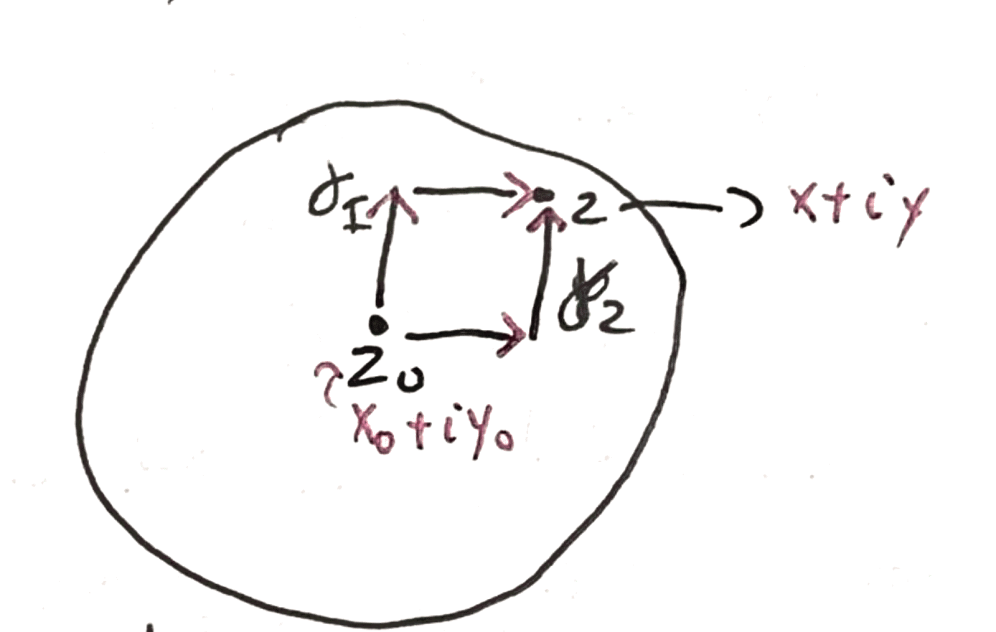
\includegraphics[width=.5\textwidth]{Figures/disk5.png}}\]
    For all $z \in \Omega$, define $F(z) = \int_{z_0}^z f(\xi) d\xi \coloneqq \int_{\gamma_1} f(z) dz = \int_{\gamma_2} f(z) dz$. We note that $F(z)$ is well-defined as Cauchy's Theorem guarantees the path-independence.\\\\
    \underline{We claim that $F \in CR^1(\Omega)$.} Indeed, tracing $\gamma_1$ and using the Fundamental Theorem of Calculus tells us that
    \[\frac{\partial F}{\partial x}(z) = f(z)\]
    Similarly, tracing along $\gamma_2$, we can parameterize $F(z)$ as
    \[F(z) = \int_{x_0}^x f(s + i y_0) ds + i \int_{y_0}^y f(x + it) dt\]
    Then it follows again that
    \[\frac{\partial F}{\partial y}(z) = i f(z)\]
    We can check that
    \[\frac{\partial F}{\partial x} + i \frac{\partial F}{\partial y} = f(z) - f(z) = 0\]
    , thus $F(z) \in CR^1(\Omega)$. Since $F(z)$ follows the Cauchy-Riemann Equations, we also know that
    \[F'(z) = \frac{1}{2}(\frac{\partial F}{\partial x} - i \frac{\partial F}{\partial y}) = \frac{1}{2}(2f(z)) = f(z)\]
    Since $F(z)$ is holomorphic, it is infinitely differentiable, so $f(z)$ is also holomorphic, so we are done.
\end{proof}

\begin{corollary}
    If $f_n \in C_z^1(\Omega)$ and $\{f_n\}$ converges to $f$ uniformly, then $f \in C_z^1(\Omega)$.
\end{corollary}

\begin{proof}
    For all sufficiently small rectangle $R$ within $\Omega$, consider
    \begin{align*}
        \int_{\partial R} f(z) dz &= \int_{\partial R} \lim_{n \to \infty} f_n dz\\
        &= \lim_{n \to \infty} \int_{\partial R} f_n dz \tag*{Uniform Convergence}\\
        &= \lim_{n \to \infty} 0 \tag*{Cauchy's Theorem}\\
        &= 0
    \end{align*}
    Thus, by Morera's Theorem, $f \in C_z^1(\Omega)$.
\end{proof}

\begin{corollary}
    If $f_n \in C_z^1(\Omega)$ and $\{f_n\}$ converges to $f$ uniformly, then $\{f_n'(z)\}$ converges to $f'(z)$ uniformly, and hence $\{f_n^{k}(z)\}$ converges to $f^{k}(z)$ uniformly.
\end{corollary}

\begin{proof}
It suffices for us to show this for the first derivative. Now for all $z \in \Omega$ and sufficiently small domain $G$, we have that
\begin{align*}
    f'(z) &= \frac{1}{2 \pi i} \int_{\partial G} \frac{f(z)}{(\xi - z)^2} d\xi \tag*{Cauchy's Formula for Derivatives}\\
    &= \frac{1}{2 \pi i} \int_{\partial G} \lim_{n \to \infty} \frac{f_n(z)}{(\xi - z)^2} d\xi\\
    &= \lim_{n \to \infty} \frac{1}{2 \pi i} \int_{\partial G} \frac{f_n(z)}{(\xi - z)^2} d\xi \tag*{Uniform Convergence}\\
    &= \lim_{n \to \infty} f_n'(z) \tag*{Cauchy's Formula for Derivatives}
\end{align*}
Thus, we have that $\{f_n'(z)\}$ converges to $f'(z)$. Since the original convergence is uniform, this convergence is also uniform.
\end{proof}

\begin{theorem}[Meta Theorem]
    Let $\phi(z, \xi): \Cbb \times X \to \Cbb$ where $X$ is some parameterization space with measure $\mu(\xi)$ that is finite, let
    $$f(z) = \int \phi(z, \xi) d\mu(\xi)$$
    Suppose $\phi$ is $CR^1$ in the variable $z$ and $f$ is bounded, then $f(z)$ is analytic.
\end{theorem}

\begin{proof}
    Since the measure $\mu$ is finite and the function is bounded, we can use Fubini's Theorem and see that, for all sufficiently small rectangles,
    \begin{align*}
        \int_R f(z) dz &= \int_R [\int \phi(z, \xi) d\mu(\xi)] dz\\
        &= \int [\int_R \phi(z, \xi) dz] d\mu(\xi) \tag*{Fubini's Theorem}\\
        &= \int 0 d\mu(\xi) \tag*{$\phi$ is $CR^1$ in the variable $z$}\\
        &= 0
    \end{align*}
\end{proof}

\begin{corollary}
    Let $f(z) = \sum_{n = 0}^\infty a_n (z - z_0)^n$ defined in $D_{z_0, r}$, then $f \in CR^1(D_{z_0, r}) = C_z^1(D_{z_0, r})$
\end{corollary}

\begin{proof}
    Let $z \in D(z_0, r)$, consider $r_1 > 0$ small enough that $cl(D(z, r_1)) \subset D(z_0, r)$, then by Heine-Cantor, we know that the partial sums
    \[\sum_{k = 0}^N a_k (z - z_0)^k \mapsto \sum_{0}^\infty a_n (z - z_0)^n \text{ converges uniformly in $D(z, r_1)$}\]
    Each of the partial sum are complex differentiable, thus by Corollary above, we have that $f \in C_z^1(D_{z_0, r})$.
\end{proof}

\begin{theorem}
    $CR^1 = C_z^1 = \text{Analytic}$
\end{theorem}

\begin{proof}
We have already shown all the directions in previous lectures and this lecture.
\end{proof}

\subsection{Power Series}

\begin{definition}
    Let $f(z) = \sum a_k (z - z_0)^k$ be a power series. We define the radius of convergence of $f$ as $R \in [0, \infty]$ such that for all $z$ such that $|z - z_0| < R$, $f(z)$ diverges, and for all $z$ such that $|z - z_0| > R$, $f(z)$ converges.
\end{definition}

\begin{remark}
    It turns out that
    \[\frac{1}{R} \coloneqq \lim \sup_{n \to \infty} |a_n|^{1/n}\]
\end{remark}

\begin{proposition}
    Let $f(z) = \sum a_k (z - z_0)^k$ be a power series with radius of convergence $R$, then $f(z)$ converges uniformly in any smaller disk of radius $r < R$ contained in $D_{z_0, R}$
\end{proposition}

\begin{proof}
    We note that $f$ is continuous on $D_{z_0, R}$, and the closure of any smaller disk is also contained in $D_{z_0, R}$, then apply Heine-Cantor.
\end{proof}

\begin{corollary}
    The following three power series:
    \begin{itemize}
        \item $\sum_{n = 0}^\infty a_n z^n$
        \item $\sum_{n = 0}^\infty n a_n z^{n-1}$
        \item $\sum_{n = 0}^\infty \frac{a_n}{n + 1} z^{n+1}$
    \end{itemize}
    all have the same radius of convergence.
\end{corollary}

\begin{proof}
    Exercise. Hint: Note that
    \[\lim_{n \to \infty} n^{1/n} = 1\]
\end{proof}

\begin{example}
    For sufficiently small $z \in \Cbb$, consider
    \[\frac{1}{1 + sin(z)} = 1 - sin(z) + sin^2(z) + ...\]
    , we can rewrite this into a power-series by noting that
    \[sin(z) = z - \frac{z^3}{3!} + \frac{z^5}{5!} + ...\]
\end{example}

\subsection{Liouville's Theorem}

\begin{theorem}
    Let $f \in Hol(\Cbb)$ be a holomorphic function on $\Cbb$, and for all $z \in \Cbb$ we have that $|f(z)| \leq M$ for some fixed $M \in \Cbb$, then $f(z)$ is identically constant.
\end{theorem}

\begin{proof}
Using Cauchy's Formula for Derivatives, we note that for all $z \in \Cbb$, for all $R > 0$,
\[f'(z) = \frac{1}{2\pi i} \int_{|\xi - z| = R} \frac{f(\xi)}{(\xi - z)^2} d\xi\]
Thus, we have that
\begin{align*}
    |f'(z)| \leq \frac{1}{2\pi} \max_{\xi \in |\xi - z|} |\frac{f(\xi)}{(\xi - z)^2}| \cdot 2 \pi R\\
    &\leq \frac{1}{2\pi} \frac{M}{R^2} \cdot 2 \pi R \tag*{Since $f$ is bounded}\\
    &= \frac{M}{R}
\end{align*}
Since this inequality holds for all $R > 0$, taking the limit as $R \to 0$, gives us that
\[|f'(z)| = 0\]
Hence $f'(z) = 0$, so
\[\frac{\partial f}{\partial z} = 0, \frac{\partial f}{\partial \overline{z}} = 0\]
So in other words
\[f_x - i f_y = 0, f_x + i f_y = 0 \implies f_x = 0, f_y = 0 \implies f(z) \text{ is constant}\]
\end{proof}

\begin{remark}
    While our Morera's Theorem applies to only triangles, up to a change of coordinate, the rectangle can really just be anything.
\end{remark}

\begin{remark}
    How to check say if $f(z) = |z|^2 = z \overline{z}$ is analytic or not? Well, we see that
    \[\frac{\partial f}{\partial \overline{z}} = \frac{\partial z}{\partial \overline{z}} \overline{z} + z \frac{\partial \overline{z}}{\partial \overline{z}} = 0 + z(1) \neq 0\]
    Thus, $f$ is not holomorphic and hence not analytic.\\\\
    Take another example, say $f(z) = |z| = (z \overline{z})^{1/2}$. This is real valued so we can use power rule and
    \[\overline{\partial}(f) = \frac{1}{2}(z \overline{z})^{-1/2} z \neq 0\]
\end{remark}

\subsection{Appendix - Cauchy–Hadamard Theorem}

In this section, we will discuss more about power series and convergence that was not covered during the lecture.

\begin{theorem}[Cauchy–Hadamard Theorem]
Consider $f(z) = \sum_{n = 0}^\infty a_n z^n$. Let $\frac{1}{0} = \infty$ and $\frac{1}{\infty} = 0$. Let $R$ be finite, non-zero, satisfying
\[\frac{1}{R} = \limsup |a_n|^{1/n}\]
Then $\sum_{n = 0}^\infty a_n z^n$ converges absolutely for $|z| < R$ and diverges for $|z| > R$. We call $R$ the \textbf{radius of convergence} and $|z| < R$ the \textbf{disc of convergence}.
\end{theorem}

% my attempt
\begin{proof}
For any $\epsilon > 0$, let $\rho \coloneqq \frac{1}{R}$.\\\\
If $|z| < R$, then there exist some $\epsilon > 0$ small enough that $|z| < \frac{1}{\rho + \epsilon} < \frac{1}{\rho} = R$. By the definition of $\limsup$ that for a sufficiently large $n$, for all $N > n$, 
\[|a_N|^{1/N} < \rho + \frac{\epsilon}{2} \ (*)\]
\begin{align*}
    |a_N z^N| &= |a_N^{1/N} z|^N\\
    &< |a_N^{1/N} \frac{1}{\rho + \epsilon}|^N \tag*{Since $|z| < \frac{1}{\rho + \epsilon}$}\\
    &< |\frac{\rho + \frac{\epsilon}{2}}{\rho + \epsilon}|^N \tag*{Using $(*)$}\\
\end{align*}
We note that $|\frac{\rho + \frac{\epsilon}{2}}{\rho + \epsilon}| < 1$ and $b_n = |\frac{\rho + \frac{\epsilon}{2}}{\rho + \epsilon}|^n$ forms a convergent geometric series. By the comparison test, we also have that $\sum_{n = N}^\infty a_n z^n$ converges, which implies that $\sum_{n = 0}^\infty a_n z^n$ converges.\\\\
If $|z| > R$, then there exist some $\epsilon > 0$ small enough that $|z| > \frac{1}{\rho - \epsilon} > \frac{1}{\rho} = R$. By the definition of $\limsup$ that for a sufficiently large $n$, for all $N > n$, 
\[|a_N|^{1/N} + \frac{\epsilon}{2} > \rho \ (*)\]
\begin{align*}
    |a_N z^N| &= |a_N^{1/N} z|^N\\
    &> |\frac{a_N^{1/N}}{\rho - \epsilon}|^N \tag*{Since $|z| > \frac{1}{\rho - \epsilon}$}\\
    &> |\frac{\rho - \frac{\epsilon}{2}}{\rho - \epsilon}|^N
\end{align*}
We note that $|\frac{\rho - \frac{\epsilon}{2}}{\rho - \epsilon}| > 1$ and $b_n = |\frac{\rho - \frac{\epsilon}{2}}{\rho - \epsilon}|^n$ forms a divergent geometric series, so the comparision test tells us that $\sum_{n = N}^\infty a_n z^n$ diverges, which implies that $\sum_{n = 0}^\infty a_n z^n$ diverges.
\end{proof}

\begin{corollary}\label{cor::radius_not_change}
Consider $f(z) = \sum_{n = 0}^\infty a_n z^n$ with radius of convergence $R > 0$, and let $g(z) = \sum_{n = 0}^\infty n a_n z^{n - 1}$. Then $g(z)$ has a radius of convergence that is also $R$.
\end{corollary}

\begin{proof}
Consider
\[\limsup_{n \to \infty} |n a_n|^{1/n} = \limsup_{n \to \infty} n^{1/n} |a_n^{1/n}|\]
It's a standard fact in real analysis that
\[\limsup_{n \to \infty} c_n b_n = \lim_{n \to \infty} c_n \limsup_{n \to \infty} b_n\]
if $\{c_n\}$ converges. We note that
\[\lim_{n \to \infty} n^{1/n} = 1\]
Since the limit exist
\[\limsup_{n \to \infty}  n^{1/n} |a_n^{1/n}| = \limsup_{n \to \infty} |a_n^{1/n}| = \frac{1}{R}\]
\end{proof}